\documentclass[obeyspaces,spaces,hyphens,handout]{beamer}
\usepackage[spanish]{babel}
\usepackage{pst-node}
\usepackage{fontspec}
\usepackage{graphicx}

%\mode<presentation>

\begin{document}
\title{Bases de datos no tradicionales - clase 3}
\author{Felipe Gorostiaga - Guido Martínez}
\institute{Bases de datos avanzadas, LCC}

\begin{frame}
  \titlepage
\end{frame}

\AtBeginSection{\frame{\sectionpage}}

\setbeamertemplate{section page}
{
	\begin{centering}
	\begin{beamercolorbox}[sep=12pt,center]{part title}
	\usebeamerfont{section title}\bf{\insertsection}\par
	\end{beamercolorbox}
	\end{centering}
}

\newcommand{\dquote}{\texttt{\char`\"}}

\section{Teorema de Brewer}

\begin{frame}
\frametitle{Introducción}
\begin{itemize}

\item	Entre las ventajas de las bases de datos no relacionales, una de las más destacadas es la facilidad de permitir a la base de datos escalar horizontalmente. \pause

\item	Sin embargo, el teorema de Brewer (o teorema CAP, por las siglas de ``Consistency, Availability y Partition tolerance'') demuestra que es imposible para un sistema de cómputo distribuido brindar justamente estas tres garantías a la vez:
		\begin{itemize}
			\item	Consistencia
			\item	Disponibilidad
			\item	Tolerancia a particionado
		\end{itemize}
		\pause
\item	Veamos cómo afecta la falta de cada una de ellas a una base de datos.

\end{itemize}
\end{frame}

\begin{frame}
\frametitle{Falta de consistencia}
\begin{itemize}

	\item	La consistencia en un sistema de base de datos distribuidos implica que todos los nodos deben visualizar los mismos datos en todo momento. \pause
	\item	Un sistema distribuido que no asegura consistencia en los datos, permite que dos consultas iguales procesadas por nodos diferentes retornen resultados diferentes. \pause
	\item	El DBMS ``Cassandra'' asegura disponibilidad y tolerancia a particionado pero no consistencia. \pause
	\item	Aunque para paliar este problema, asegura ``consistencia eventual'', que garantiza que si no hay nuevas actualizaciones de un dato, eventualmente todos los accesos a él retornarán el mismo valor (actualizado).

\end{itemize}
\end{frame}

\begin{frame}
\frametitle{Falta de disponibilidad}
\begin{itemize}

	\item	La disponibilidad de una base de datos requiere que todas las transacciones sean procesadas y respondidas por el sistema. \pause
	\item	Un sistema que no asegure disponibilidad completa hará que sus usuarios en algún momento no puedan acceder ni actualizar los datos en ellas almacenados, aunque sea por un corto período de tiempo.
	\item	Los DBMS que utilizan la famiila de protocolos Paxos para concurrencia (e.g. Neo4j) no pueden asegurar una disponibilidad del 100\%

\end{itemize}
\end{frame}

\begin{frame}
\frametitle{No tolerancia al particionado}
\begin{itemize}

	\item	El particionado de un conjunto de nodos se refiere a una falla que impide que un conjunto de ellos no pueda comunicarse con los restantes (los particiona). \pause
	\item	Tolerar el particionado significa que la base de datos seguirá funcionando a pesar de que haya fallas de comunicación entre los subsistemas. \pause
	\item	No tolerarlo, implica que la base de datos puede no operar si algunos de sus nodos fallan. \pause
	\item	Las bases de datos relacionales no toleran el particionado del sistema.
	
\end{itemize}
\end{frame}

\begin{frame}
\frametitle{¿Por qué?}
\begin{itemize}

	\item TODO
\end{itemize}
\end{frame}


\section{Bases de datos orientadas a Grafos (BDOG o Graph Databases)}

\begin{frame}
\frametitle{Introducción}
\begin{itemize}

\item	Algunas aplicaciones requieren guardar grafos gigantescos de
	forma segura y manipularlos eficientemente.
	\pause

\item	Como siempre, se puede usar un motor relacional y manejar
	la lógica a nivel de aplicación. Se podrían incluso usar índices
	para acelerar los joins (que representarían la búsqueda de vecinos)
	a costo de updates mas lentos y espacio en disco.
	\pause

\item	Una BDOG se define como una base de datos que provee ``adjacencia
	sin uso de índices'', o sea, que maneja los grafos de una manera
	\textit{natural} y \textit{eficiente}.
	\pause

\item	De esta manera, se prestan a modelar datos heterogéneos y
	conectados.
\end{itemize}
\end{frame}

\begin{frame}
\frametitle{Un poco de autobombo}
\begin{itemize}
\item	We live in a connected world. There are no isolated pieces of
	information, but rich, connected domains all around us. Only a database
	that embraces relationships as a core aspect of its data model is able
	to store, process, and query connections efficiently. \textbf{While other
	databases compute relationships expensively at query time, a graph
	database stores connections as first class citizens, readily available
	for any “join-like” navigation operation.} Accessing those already
	persistent connections is an efficient, constant-time operation and
	allows you to quickly traverse millions of connections per second per
	core.
\end{itemize}
\end{frame}

\begin{frame}
\center
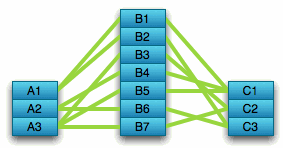
\includegraphics[width=0.9\linewidth,height=0.9\textheight,keepaspectratio]{bdog-1}
\end{frame}
\begin{frame}
\center
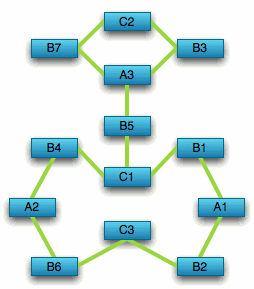
\includegraphics[width=0.9\linewidth,height=0.9\textheight,keepaspectratio]{bdog-2}
\end{frame}

\begin{frame}
\frametitle{Implementando un KV store}
 \center
 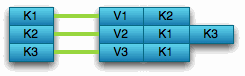
\includegraphics[width=0.9\linewidth,height=0.9\textheight,keepaspectratio]{bdog-3}
\end{frame}

\begin{frame}
\frametitle{Implementando un KV store}
 \center
 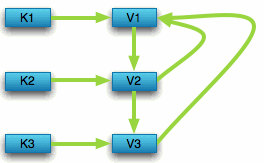
\includegraphics[width=0.9\linewidth,height=0.9\textheight,keepaspectratio]{bdog-4}
\end{frame}

\begin{frame}
\frametitle{Características}
\begin{itemize}
\item	En una BDOG, nunca puede haber una relación sin ambos nodos
	que conecta (\textit{No broken links}).
	\pause

\item	Pueden tener consistencia ACID (Neo4j la tiene).
\end{itemize}
\end{frame}

\section{Neo4j}

\begin{frame}
\frametitle{Neo4j}
\begin{itemize}
\item	Neo4j es un GDBMS open-source, con una versión gratuita y una
	paga, que implementa este modelo.
	\pause

\item	Usada por muchísimas empresas y organizaciones (eBay, Walmart,
	Cisco, y más).
\end{itemize}
\end{frame}


\begin{frame}
\frametitle{Bibliografía}
\begin{itemize}
	\footnotesize
	\item \url{http://neo4j.com/developer/graph-database/}
\end{itemize}
\end{frame}

\begin{frame}
\begin{center}
	¿Dudas?
	\pause

	¿Quejas?
\end{center}
\end{frame}

\end{document}
